%!TEX root = ../../main.tex
\chapter{Verwendung von Geräteschnittstellen}

Eine weitere Eigenschaft von PWAs ist der Zugriff auf Geräteschnittstellen. Um dies zu zeigen, wurde die Geolocation- und Kameraschnittstelle implementiert.
Wird in der unteren Navigationsleiste das mittlere Symbol ausgewählt, nutzt die Webanwendung die Geolocation-Schnittstelle um den Anwender sein Breiten- und Längengrad mitzuteilen. Da es sich hierbei um eine datenschutzkritische Funktion handelt, muss der Anwender die Erlaubnis erteilen, den Standort zu teilen. 

Die Geolocation wird auf allen Plattformen korrekt angezeigt und wird exemplarisch im IOS-System auf folgenden Abbildungen \ref{img:geo1} und \ref{img:geo2} gezeigt. 

\begin{figure}[!htb]
    \begin{minipage}[b]{.4\linewidth} % [b] => Ausrichtung an \caption
       \includegraphics[width=\linewidth]{Iphone05.PNG}
       \caption{Einholen der Nutzererlaubnis für den Zugriff auf den aktuellen Standort}
       \label{img:geo1}
    \end{minipage}
    \hspace{.1\linewidth}% Abstand zwischen Bilder
    \begin{minipage}[b]{.4\linewidth} % [b] => Ausrichtung an \caption
       \includegraphics[width=\linewidth]{iphone06.PNG}
       \caption{Darstellung des aktuellen Standortes in einer IOS-Anwendung}
       \label{img:geo2}
    \end{minipage}
 \end{figure}

 Die Anwendung implementiert auch die Kameraschnittstelle welche auch auf allen Plattformen, die auf eine Kamera zugreifen können funktioniert. Der Anwender muss auch für diese Funktion sein Einverständnis geben. Die Kamera Funktion ist Kamerea-Icon in der unteren Navigationsleiste erreichbar und ist in den folgenden Abbildungen \ref{img:Kamera1} und \ref{img:Kamera2} unter IOS dargestellt.

 \begin{figure}[!htb]
    \begin{minipage}[b]{.4\linewidth} % [b] => Ausrichtung an \caption
       \includegraphics[width=\linewidth]{Iphone07.PNG}
       \caption{Einholen der Nutzererlaubnis für den Zugriff auf die Kamera}
       \label{img:Kamera1}
    \end{minipage}
    \hspace{.1\linewidth}% Abstand zwischen Bilder
    \begin{minipage}[b]{.4\linewidth} % [b] => Ausrichtung an \caption
       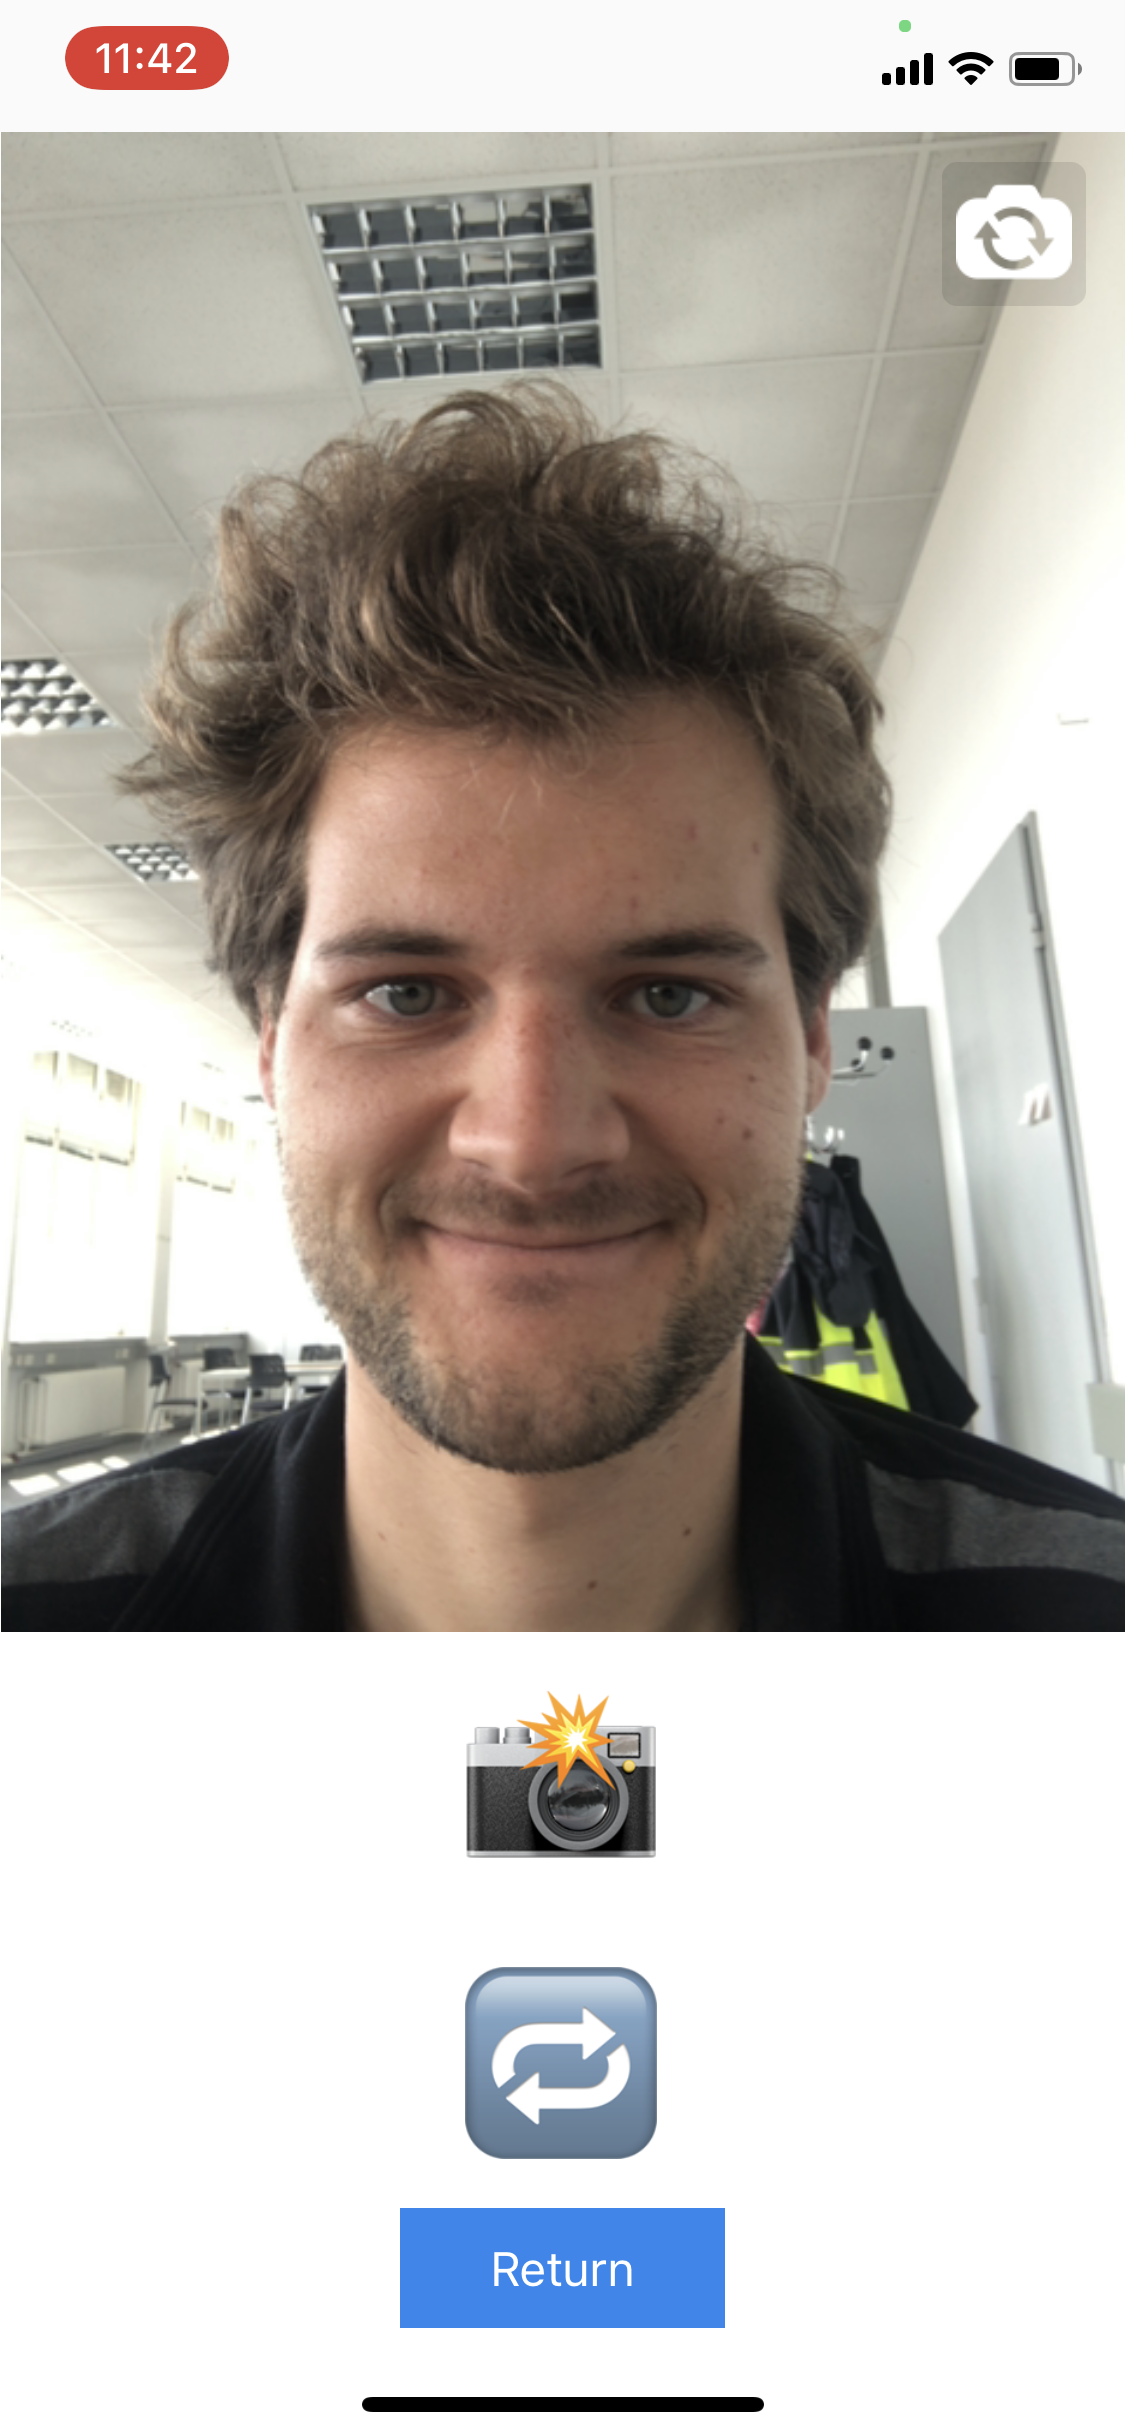
\includegraphics[width=\linewidth]{iphone08.PNG}
       \caption{Darstellung der Kamera-Funktion unter IOS}
       \label{img:Kamera2}
    \end{minipage}
 \end{figure}


